\documentclass{ctexart}
\usepackage{geometry}
\usepackage{diagbox}
\usepackage{graphicx}
\usepackage{subfigure}
\usepackage{amsmath}
\usepackage{amssymb}
\usepackage{indentfirst}
\usepackage{xfrac}
\usepackage{color}
\usepackage[table]{xcolor}
\usepackage{multirow}
\usepackage{titlesec}
\usepackage{bm}
\usepackage{caption}
\usepackage{booktabs}
\usepackage{ulem}
\usepackage{float}
% 调节页边距
\geometry{a4paper,left=3cm,right=3cm,top=3cm,bottom=3cm}
% 调节摘要
\renewcommand{\abstractname}{\large 摘要\\}
\title{\textbf{UP主粉丝数的影响因素分析}}
\author{\textbf{Group 2 周子逸\ 徐智昱\ 逄一哲\ 祝尔康}}
\date{}
\begin{document}
\maketitle
%------------------------------------摘要------------------------------------
\begin{abstract}
    本文基于逻辑回归课上学习的多分类数据分析方法,对B站UP主粉丝数的影响因素进行分析。
本文从ifans网站抽取B站UP主的粉丝数、性别、分区等相关数据,将UP主按照粉丝数分为4个水平,
通过EDA总结变量特点并初步筛变量,之后分别使用列联表卡方检验、对数线性模型、多分类
逻辑回归模型对数据进行分析解释,探究了UP主粉丝数水平与性别、分区、视频数等变量的关系,
并试图结合各个模型对有意愿成为UP主的同学提供有关建议。
\end{abstract}
%------------------------------------目录------------------------------------
\tableofcontents
%------------------------------------正文------------------------------------
\newpage
\section{背景介绍}
Bilibili视频网站(下文简称B站)在近年愈发受到年轻人的欢迎,数量庞大的UP主群体为B站的视频生态的多样性做出了
非常大的贡献。在庞大的UP主群体之下,UP主的粉丝数也有显著的差异。本研究旨在通过研究各种影响因素与UP主的粉丝
数量的分层不同带来的影响。\\
\indent 本次研究的数据来源于ifans网站,网站上提供了粉丝量、最近更新时间、分区、视频数、
充电数、近8篇平均视频投币数、近8篇平均视频弹幕数、近8篇平均视频收藏数、近8篇平均视频点赞数、
近8篇平均视频播放数、近8篇平均视频评论数、近8篇平均视频分享数数据、性别数据,本研究将所有变量均放入模型中进行研究,
同时研究是否能够有减少变量的方法。本研究凭借网站上的粉丝数量分区,
将粉丝量的分区分为“<10万”,“10万~50万”,“50万~100万”,“>100万”四个分区,作为后续分类型数据分析的基础。\\
\indent 由于不同分区的UP主人数差异较大,本研究采用回溯性研究方法,即在四个粉丝量的分区分别抽取250个UP主的数据
进行研究分析。

\section{数据爬取与预处理}

分别选择粉丝数量为10万以内、10万到50万、50万到一百万以及粉丝数量一百万以上的up主,排序方式使用
随机排序,各采样500个up主(网页查询上限就是500)。然后利用singleFile插件将网页中需要爬取的内容
选中,保存为html文件。接着,利用rvest对html文件进行爬取,并将四种粉丝量的up主的数据分别整理为
xlsx格式并与原始网页进行比对,检查爬取过程中是否出现错误。然后,分别读入4个xlsx格式的文件,剔
除缺失性别等信息的数据,然后在各个粉丝档次剩下的up主中随机采样,样本量为250。最终将1000个up主
的数据整理在一起,就得到了大作业所用的数据集。在数据爬取的过程中遇到了一些困难,例如up主昵称没
法爬取,最后采用了手动复制的方法解决。

由于每个变量的单位相差较大,为了避免单位造成的影响,本研究将所有非分类型数据进行归一化处理。
由于选择的解释变量均为非负数据,为保持这一性质,采用以下的归一化方法。
\begin{equation}
    \tilde{x} = \frac{x-\alpha}{\beta - \alpha}
\end{equation}
其中$\alpha$,$\beta$分别为本解释变量中的最大值与最小值。

\section{探索性数据分析}
\subsection{数据可视化}

首先,作出各类数据之间相关系数的热量图:

\begin{figure}[H]
    \centering
    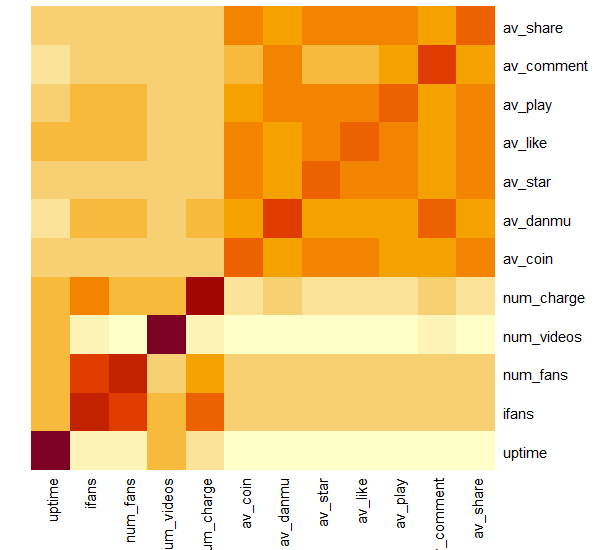
\includegraphics[width=0.40\textwidth]{EDA/Heatmap.png}
    \caption{Heatmap for Correlation}
\end{figure}

由热量图可见,右上角各种平均的线性相关性较强。由于作出Scatter Plot Matrix时,如果变量过多,则容易显示不清楚,因此
选择近8篇平均投币数和近8篇平均点赞数作为各种平均的代表绘制Scatter Plot Matrix。

\begin{figure}[H]
    \centering
    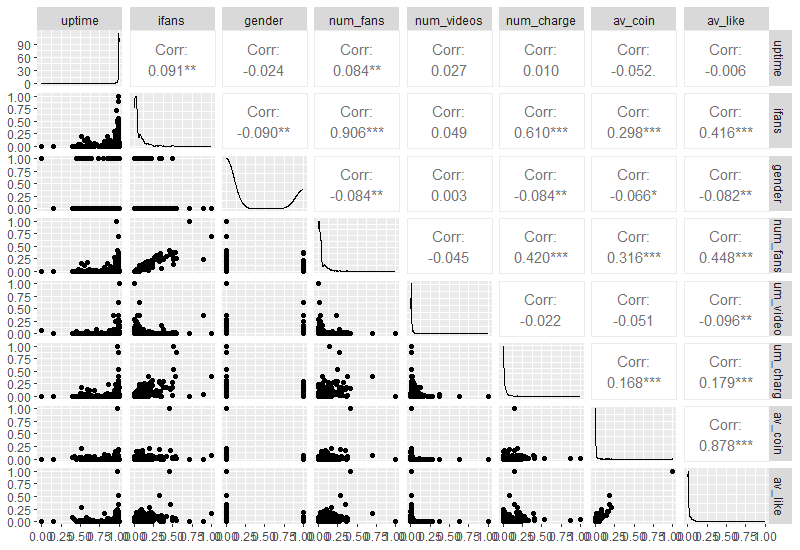
\includegraphics[width=0.60\textwidth]{EDA/Spm.png}
    \caption{Scatter Plot Matrix}
\end{figure}

由Scatter Plot Matrix可见,各类数据间普遍具有一定的相关性,这说明对这些数据建立模型进行分析应该会有一定的效果。同时,由每个变量的核密度
估计可见,各个解释变量是明显右偏的,这说明B站的UP主存在一定的少部分UP主占据了极大的资源的效应。\\

通过Scatter Plot Matrix,作出两大分区变量粉丝量与性别和与这两个因素有显著作用的的变量之间的箱型图,观察这些因素对
两大分类型变量的影响。

\begin{figure}[H]
    \centering
    \begin{minipage}[t]{0.48\textwidth}
        \centering
        \includegraphics[width=\textwidth]{EDA/av_like_gender_boxplot.png}
        \caption{各性别平均点赞数}
    \end{minipage}
    \begin{minipage}[t]{0.48\textwidth}
        \centering
        \includegraphics[width=\textwidth]{EDA/num_charges_gender_boxplot.png}
        \caption{各性别充电数}
    \end{minipage}
\end{figure}

\begin{figure}[H]
    \centering
    \begin{minipage}[t]{0.48\textwidth}
        \centering
        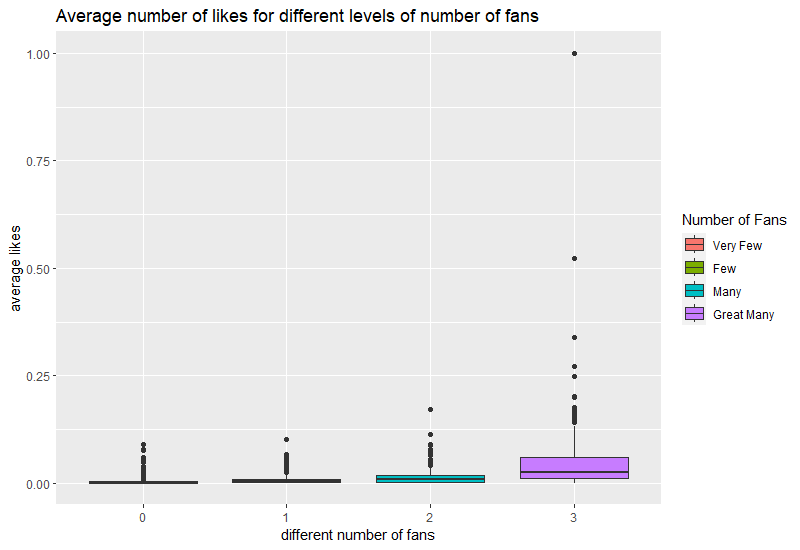
\includegraphics[width=\textwidth]{EDA/av_like_fans_boxplot.png}
        \caption{各粉丝量平均点赞数}
    \end{minipage}
    \begin{minipage}[t]{0.48\textwidth}
        \centering
        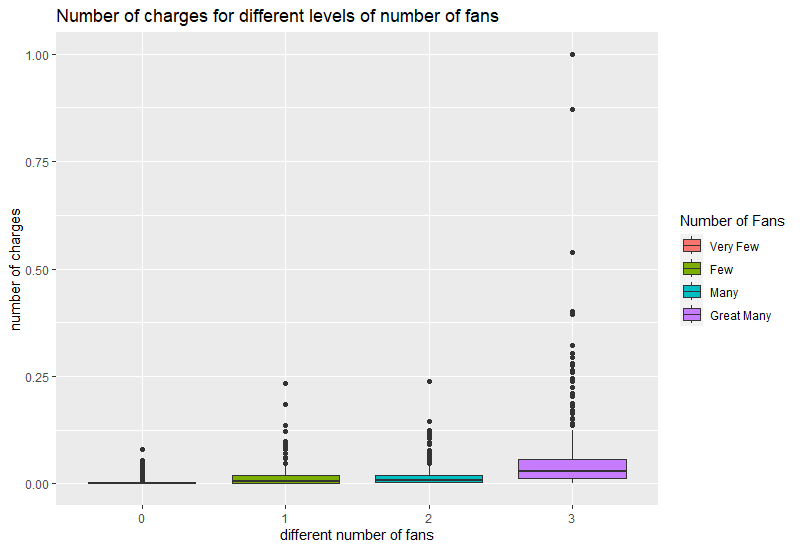
\includegraphics[width=\textwidth]{EDA/num_charge_fan_boxplot.png}
        \caption{各粉丝量充电数}
    \end{minipage}
\end{figure}

由图可见,对于部分解释变量,其对不同性别确实有显著的影响;对于平均点赞数和充电数而言,均表现为男性的
离群值点远大于女性的特点。而诸多解释变量对于粉丝量也有显著的作用,与上述分析相似的,对于粉丝量较少的三类,实际上
两个变量的表现较为相似,而粉丝量大于100万的样本,在点赞量和充电数上,无论是平均值还是数量高的值都明显多于前三类。
这映照了之前认为的少部分UP主获得了最多的关注的同时,也按时是否需要优化分区结构,能够获得更好的效果。

由于解释变量仍较多,并且从Scatter Plot Matrix可以看出部分解释变量之间存在较为显著的线性相关性,
因此考虑是否能对解释变量进行一定程度的筛选。下面考虑利用主成分分析(PCA)和LASSO两种方法对是否能够减少解释变量数量进行分析。

\subsection{主成分分析}
对归一化后的连续型解释变量进行主成分分析,所得肘图如下图:
\begin{figure}[H]
    \centering
    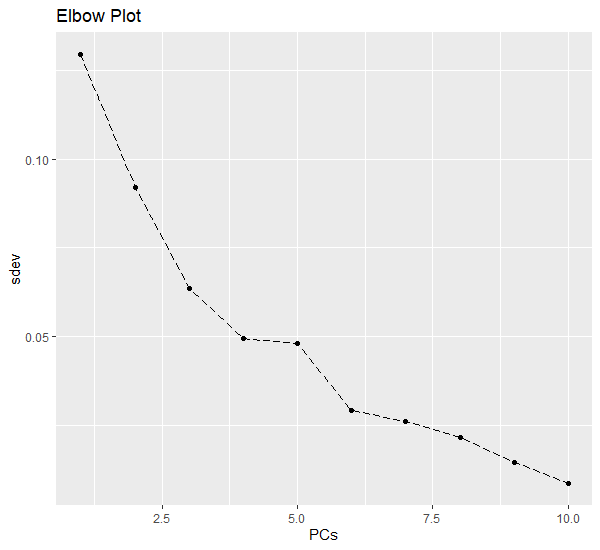
\includegraphics[width=0.45\textwidth]{EDA/PCA_elbow.png}
    \caption{PCA肘图}
\end{figure}

由肘图可见,实际上PCA的效果并不好,在拐点后方程下降速度仍较为显著,
并且拐点处的方差仍较大。如果要保留99\%的信息量,则可舍弃最后两个主成分;如果要保留95\%的信息量,则可舍弃最后四个主成分。一定程度上起到了降维
的效果。PCA的旋转矩阵如下表:
\begin{table}[H]
    \centering
    \begin{tabular}{|c|c|c|c|c|c|c|c|c|c|c|}
    \hline
            & PC1   & PC2   & PC3   & PC4   & PC5   & PC6   & PC7   & PC8   & PC9   & PC10  \\ \hline
    uptime  & -0.17 & 0.97  & 0     & 0.11  & -0.08 & 0.04  & -0.03 & 0.01  & -0.02 & -0.01 \\ \hline
    videos  & -0.04 & 0     & -0.03 & 0.55  & 0.83  & -0.04 & -0.04 & 0     & -0.01 & 0.01  \\ \hline
    charge  & 0.15  & 0.07  & -0.93 & -0.29 & 0.17  & 0.04  & -0.01 & 0     & -0.01 & 0     \\ \hline
    coin    & 0.23  & 0.07  & 0.08  & -0.07 & 0.1   & 0.21  & 0.46  & -0.36 & 0.33  & -0.65 \\ \hline
    danmu   & 0.51  & 0.01  & -0.17 & 0.57  & -0.35 & -0.19 & 0.37  & 0.3   & -0.01 & 0.08  \\ \hline
    star    & 0.3   & 0.08  & 0.16  & -0.2  & 0.16  & 0.09  & 0.31  & -0.26 & -0.78 & 0.17  \\ \hline
    like    & 0.32  & 0.12  & 0.14  & -0.19 & 0.14  & -0.13 & 0.09  & -0.32 & 0.51  & 0.65  \\ \hline
    play    & 0.48  & 0.12  & 0.14  & -0.19 & 0.11  & -0.58 & -0.47 & 0.06  & -0.05 & -0.35 \\ \hline
    comment & 0.31  & -0.03 & -0.07 & 0.33  & -0.21 & 0.49  & -0.56 & -0.44 & -0.05 & 0.01  \\ \hline
    share   & 0.34  & 0.08  & 0.2   & -0.23 & 0.2   & 0.56  & -0.07 & 0.65  & 0.1   & 0.03  \\ \hline
    \end{tabular}
    \caption{PCA旋转矩阵}
\end{table}

由旋转矩阵可见,实际上PCA的解释性较差。又由于本研究主要为解释性研究,因此如果采用PCA后的主成分进行分析,
最后会导致解释性较差,所以将舍弃PCA部分的结果。

\subsection{LASSO}
利用LASSO将所有解释变量放入模型中,分别对粉丝量(分类型)作多分类变量逻辑回归与对粉丝量(连续型)作广义线性回归,得到
均方误差随正则项的变化分别如下两图。
\begin{figure}[H]
    \begin{minipage}[t]{0.48\textwidth}
        \centering
        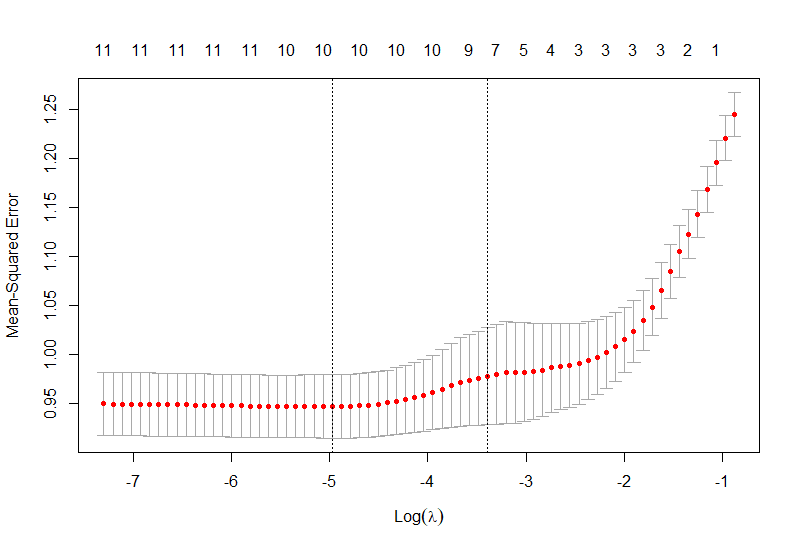
\includegraphics[width=\textwidth]{EDA/lasso_multinomial.png}
        \caption{多分类逻辑回归}
    \end{minipage}
    \begin{minipage}[t]{0.48\textwidth}
        \centering
        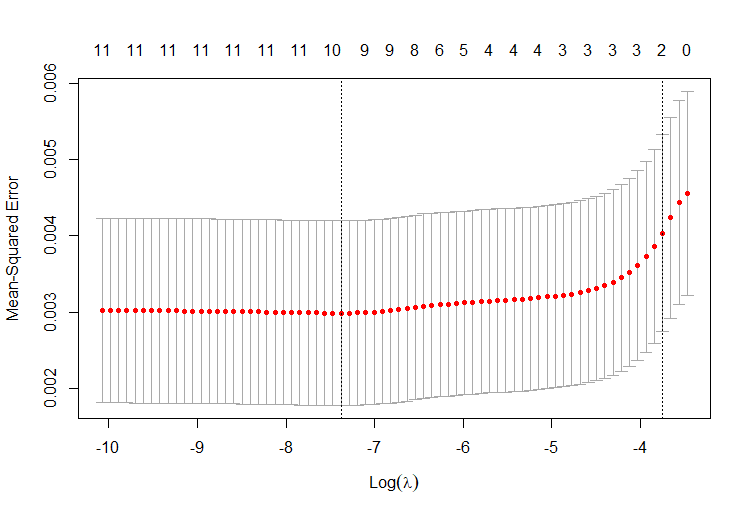
\includegraphics[width=\textwidth]{EDA/lasso_continuous.png}
        \caption{连续型线性回归}
    \end{minipage}
\end{figure}

所得在让均方误差最小的正则项系数与在1个标准差意义下的正则项系数如下表,其中进行多分类逻辑回归得到4个返回的$\lambda$值,
筛选出效果较好的值对应的系数:

\begin{table}[H]
    \centering
    \begin{tabular}{ccccc}
    \hline
    \multirow{2}{*}{Name} & \multicolumn{2}{c}{Multinomial} & \multicolumn{2}{c}{Continuous} \\ \cline{2-5} 
                          & min            & 1se            & min            & 1se           \\ \hline
    Intercept             & 8.76           & 5.26           & -0.03          & 0.04          \\
    uptime                & -8.16          & -5.69          & 0.05           & 0             \\
    gender                & 0.08           & 0.15           & 0              & 0             \\
    videos                & -1.08          & 0              & 0              & 0             \\
    charge                & -54.93         & -20.74         & 0.34           & 0.05          \\
    coin                  & 0              & 0              & -0.3           & 0             \\
    danmu                 & 0              & 0              & 0.09           & 0             \\
    star                  & 8.08           & 0              & -0.11          & 0             \\
    like                  & -73.91         & -21.17         & 0.66           & 0             \\
    play                  & -13.79         & 0              & 0.2            & 0.1           \\
    comment               & -1.07          & 0              & -0.06          & 0             \\
    share                 & 22.47          & 0              & -0.16          & 0             \\ \hline
    \end{tabular}
    \caption{正则后系数表}
\end{table}

由上表可见,使用LASSO多类别逻辑回归和线性回归得到的系数有较为明显的区别,因此说明经过将粉丝量分类,得到了
不同的回归结果,有不同的解释效应。因此,在进行多分类逻辑回归会得到直接线性回归不同的结果。由于两个1个标准差内的结果
都省略了过多的变量,可能造成解释能力不足,因此在进行多分类逻辑回归时,考虑舍弃投币数和弹幕数两个变量。

\section{列联表分析}

为了探索UP主粉丝数水平与分区和性别的关系,我们对其构成的三维列联表尝试了卡方检验、累计
逻辑回归和log linear model,得到了三个有意义的结论。

\subsection{列联表卡方检验}

首先我们利用pearson检验分别对无分区变量的总表和考虑分区的三个子表测试变量间的独立性。在
总表中得到的卡方值为$10^{-16}$,说明粉丝数水平与性别显著相关;在动画、游戏区中的卡方值分别为
$0.6172,\ 0.4575$,这说明可以认为粉丝数水平和性别独立;而在知识分区中卡方值则为0.02,这说
明有$95\%$以上的把握认为粉丝数水平与性别有关。

\subsection{累积逻辑回归模型}

为了更好地利用粉丝数水平作为次序变量的特点,我们采用了适用于这种情形的累积逻辑回归模型。
下面多分类逻辑回归部分也会使用到该模型,区别在于后面针对的解释变量更多且大多为连续型,
而本处的解释变量是性别和分区两个分类型变量。

模型的响应变量为Fanslevel,是一个ordinal的变量,代表up主粉丝数水平类别,分为4类,“<10w”、“10w-50w”
”、“50w-100w”、“>100w”分别规定为$j=1,2,3,4$,这里“>100w”默认为1,所以j只可能取1,2,3。解释变量为性别和分区,
其中性别变量gender是一个binary的变量,1代表女性,0代表男性;分区我们考虑了知识区、动画区和游戏区,
使用type1和type2两个哑变量来表示分区变量,(type1,type2)=(0,0)对应知识区,(type1,type2)=(1,0)对应动画区,
(type1,type2)=(0,1)对应游戏区。全模型如下:
\begin{equation*}
    \operatorname{logit}[P(fanslevel≤j|type)]=\alpha_j+\beta_g*gender+\beta_1*type1+
    \beta_2*type2+\beta_{g1}*gender*type1+\beta_{g2}*gender*type2
\end{equation*}

对于全模型,我们求得各参数分别为:$\alpha_1=1.844,\alpha_2=3.467,\alpha_3=4.346,\beta_g=0.049,
\beta_1= 0.145, \beta_2=0.270, \beta_{g1}=-0.006=7, \beta_{g2}=-0.087$。但是只有截距项和$\beta_1, \beta_2$
较为显著。我们利用drop1函数比较AIC来减少模型中的变量数,并利用anova来检验丢弃变量操作的合理性。
最终我们选定只有type1和type2两个解释变量的模型
$$\operatorname{logit}[P(fanslevel≤j|type)]=\alpha_j+\beta_1*type1+\beta_2*type2$$
模型残差为$14.700$,与全模型做方差分析得到p值为$0.513$,说明简化模型并未损失太多信息。简化后
的各参数分别为:$\alpha_1=1.858,\ \alpha_2=3.481,\ \alpha_3=4.360,\ \beta_1= 0.144,\ \beta_2=0.248$。该模型中
性别和性别的交互项都不显著与我们此前的列联表卡方检验结果相呼应,表明性别在各个
分区看来不是一个粉丝数水平的显著决定因素,此前不考虑分区的结果正是明显的辛普森
悖论现象。

对于$\beta_1$的理解为:$\operatorname{logit}[P(fanslevel≤j|type1=1)]-\operatorname{logit}
[P(fanslevel≤j|type1=0)]=0.144$,即fanslevel关于type1的odds ratio为$1.155$。这表明在动画区的某一粉丝数水
平(水平$j$)以下的概率对应的odds,为在知识区的同一粉丝数水平(水平$j$)以下的概率对应
odds的$1.155$倍,这反映了在动画区聚集在相对低级粉丝数水平的up主比例高于知识区。同理,

对于$\beta_2$的理解为:$\operatorname{logit}[P(fanslevel≤j|type2=1)]-\operatorname{logit}
[P(fanslevel≤j|type2=0)]=0.248$,即fanslevel关于type1的odds ratio为$1.281$。这
表明在游戏区的某一粉丝数水平(水平$j$)以下的概率对应的odds,为在知识区的同一粉丝数水平(水平$j$)以下的概率对应odds的$1.281$倍,
这反映了在游戏区聚集在相对低级粉丝数水平的UP主比例高于知识区。因为$\beta_2>\beta_1$,我们可以
进一步认为在游戏区聚集在相对低级粉丝数水平的UP主比例高于动画区,这意味着游戏区
竞争更为激烈。

观察实际的各UP主分布情况如下表所示,可以看出实际情况确实如此,但与低粉丝数UP主
比例高相对应的是游戏区各水平UP主的数目都明显多于动画、知识分区,这一点将在
log linear model中进一步体现。

\begin{table}[H]
    \centering
    \begin{tabular}{ccccc}
        \toprule
         动画区粉丝数占比 & <10w & 10w-50w & 50w-100w & >100w  \\
        \midrule
         所占比例 & 0.881 & 0.093 & 0.0148 & 0.011 \\
        \bottomrule
    \end{tabular}
    \caption{动画区各粉丝数水平占比}
\end{table}
\begin{table}[H]
    \centering
    \begin{tabular}{ccccc}
        \toprule
         游戏区粉丝数占比 & <10w & 10w-50w & 50w-100w & >100w  \\
        \midrule
         所占比例 & 0.892 & 0.085 & 0.013 & 0.010 \\
        \bottomrule
    \end{tabular}
    \caption{游戏区各粉丝数水平占比}
\end{table}
\begin{table}[H]
    \centering
    \begin{tabular}{ccccc}
        \toprule
         知识区粉丝数占比 & <10w & 10w-50w & 50w-100w & >100w  \\
        \midrule
         所占比例 & 0.865 & 0.015 & 0.0148 & 0.011 \\
        \bottomrule
    \end{tabular}
    \caption{知识区各粉丝数水平占比}
\end{table}

\subsection{对数线性模型}

为充分利用UP主粉丝数是count型变量的特点以及分区和性别两个解释变量之间可能存在的关系,
考虑使用log linear model进行建模。 模型如下:
\begin{equation}
    \log(\mu_{ijk})=\lambda+\lambda_i^X+\lambda_j^Y+\lambda_k^Z+\lambda_{ij}^{XY}
    +\lambda_{jk}^{YZ}+\lambda_{ki}^{ZX}+\lambda_{ijk}^{XYZ}
\end{equation}

其中$X,\ Y,\ Z$分别对应粉丝数水平fanslevel,性别和分区,各参数含义如下:

\begin{table}[H]
    \begin{tabular}{cl}
        \toprule
          参数名 & 参数含义  \\
        \midrule
          $\lambda$ & 截距项,代表基线水平。这里基线为50w-100w粉丝量的动画区男性up主 \\
          $\lambda_i^X$ & 单独代表X(粉丝量水平)对人数的作用效果,“<10w”“10w-50w”“50w-100w”“>100w”\\
                        & 分别规定为$j=1,2,0,3$,对应为little,middle,big,superbig,这里以big为基线水平。\\
          $\lambda_j^Y$ & 单独代表Y(性别)对人数的作用效果,$j=0,1$分别代表男性,女性\\
          $\lambda_k^Z$ & 单独代表Z(分区)对人数的作用效果,动画、游戏、知识区分别对应$Z=0,1,2$。动画区\\
                        & 为基线水平。\\
          $\lambda_{ij}^{XY}$ & 代表粉丝量水平、性别变量的协同作用效果\\
          $\lambda_{jk}^{YZ}$ & 代表性别、分区变量的协同作用效果\\
          $\lambda_{ki}^{ZX}$ & 代表粉丝量水平、分区变量的协同作用效果\\
          $\lambda_{ijk}^{XYZ}$ & 代表粉丝量水平、性别和分区变量的协同作用效果\\
        \bottomrule
     \end{tabular}
    \caption{对数线性模型的参数解释}
\end{table}

认为下标出现$0$的系数对应为$0$,如$\lambda_0^X=\lambda_j^Y=\lambda_k^Z=\cdots=0$。
由于全模型过于复杂,我们利用drop1函数在AIC减小不是很大的情况下删除了三交互项
($\lambda_{ijk}^{XYZ}$)和性别与粉丝数水平的二交互项($\lambda_{ij}^{XY}$),最终模型仅剩15个参数,
参数估计如下:
\begin{table}[H]
    \centering
    \begin{tabular}{cccccccc}
        \toprule
        $\lambda$ & $\lambda_1^X$ & $\lambda_2^X$ & $\lambda_3^X$ & $\lambda_1^Y$ 
        & $\lambda_1^Z$ & $\lambda_2^Z$ & $\lambda_{11}^{XZ}$ \\
        \midrule
        5.0 & 4.1 & 1.8 & -0.3 & -0.7 & 0.7 & 0.4 & 0.1\\
        \midrule  
        $\lambda_{21}^{XZ}$ & $\lambda_{31}^{XZ}$ & $\lambda_{12}^{XZ}$ & $\lambda_{22}^{XZ}$ & 
        $\lambda_{32}^{XZ}$ & $\lambda_{11}^{YZ}$ & $\lambda_{12}^{YZ}$ & \\
        \midrule
        0.002 & -0.02 & -0.2 & -0.05 & -0.06 & -5.4 & -0.2 & \\
        \bottomrule
    \end{tabular}
    \caption{对数线性模型的拟合参数}
\end{table}


所有变量参数中,截距项为$\lambda$;所有粉丝数水平变量$\lambda_1^X,\ \lambda_2^X,\ \lambda_3^X$;
所有性别变量$\lambda_1^Y$;所有分区变量$\lambda_1^Z、\lambda_2^Z$;小粉丝量水平和知识分区的二交互
项$\lambda_{12}^{XZ}$;所有性别和分区的二交互项$\lambda_{11}^{YZ}$,$\lambda_{12}^{YZ}$均效应显著。
利用R进行检验,该模型拟合效果很好,最大的标准化残差只有$2.93$。但若进一步删除不显著的变量,1/3的拟合
结果会出现绝对值大于3的标准残差。

\begin{figure}[H]
    \centering
    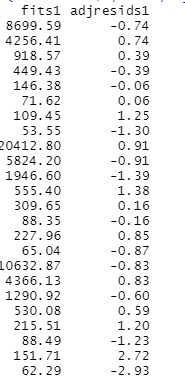
\includegraphics[]{LLM/LLM_fit.png}
    \caption{对数线性模型拟合结果}
\end{figure}

三交互项参数的不显著说明模型三个变量具有同质性,即任意两个变量的odds ratio不受
第三个变量的影响;性别与粉丝数水平二交互项参数的不显著说明在给定分区的情况下两
个变量间是独立的,这与累计逻辑回归的结论是一致的;粉丝量水平与知识分区的二交互
项中仅有小粉丝量水平和知识分区的二交互项显著,且参数绝对值普遍较小,这说明在给定
性别的情况下,除了知识区的小粉丝量和大粉丝量水平UP主数目有明显差异,其他都区别不
大。

继续观察各参数的正负,我们可得到以下结论:

(1) 小、中粉丝量水平(<10w和10w-50w)参数为正,超大粉丝量水平(>100w)参数为负。
这说明性别、分区固定时,粉丝数越多的up主对应的人数越少,呈单调递减。

(2) $\lambda_1^Y<0$,这反映了男性UP主数量明显多于女性UP主。

(3) $\lambda_1^Z=0.749>\lambda_2^Z=0.387>0$,这说明游戏分区人数>知识分区人数>动画分区人数。

(4) 小粉丝量水平和知识分区的二交互项系数为$-0.186108<0$,说明:(\romannumeral1) 固定
分区为知识区和性别时、<10w粉丝数水平相比50w-100w水平UP主约为$0.83$倍;(\romannumeral2) 或
者固定性别、固定粉丝数水平为<10w,知识分区该类UP主人数约为动画分区的0.83倍。

(5) 性别和游戏分区的二交互项系数为$-0.539<0$,说明:(\romannumeral1) 固定性别为
女和粉丝数水平时,游戏分区该类UP主的数目约为动画分区的$0.58$倍;(\romannumeral2) 
固定分区为游戏分区并固定粉丝数水平时,女性UP主中的该类别UP主为男性中该类UP主的$0.58$倍。

(6) 性别和知识分区的二交互项系数为$-0.175<0$,说明:(\romannumeral1)固定性别为女
和粉丝数水平时,知识分区中该类UP主数目为动画分区中的$0.84$倍;(\romannumeral2) 固
定在知识分区并固定粉丝数水平,女性UP主中该类别UP主数目为为男性中该类UP主的$0.84$倍。


\section{多分类逻辑回归分析}

为了分析性别以及点赞数、充电数这些连续型变量与UP主粉丝数分区的关系,我们采用多分类
逻辑回归模型进行建模分析。

\subsection{变量选取}

根据前面部分可知,我们按照“<10万”,“10万~50万”,“50万~100万”,“>100万”的标准将up
主按照粉丝数分成了4类,我们将这4个UP主量级分别记为小UP主,中UP主,大UP主和超级UP主,
得到响应变量如下:
\begin{table}[H]
    \centering
    \begin{tabular}{ccc}
        \toprule
         响应变量 & 变量类型 & 变量含义  \\
        \midrule
         fans\_cat & Multicategory & 粉丝数的分类,small, middle, big, super big四类 \\
        \bottomrule
    \end{tabular}
    \caption{多分类逻辑回归响应变量}
\end{table}

对于解释变量,我们一共有1个二分类的性别变量和9个归一化后的连续型变量,各个
变量的含义如下标所示,根据LASSO部分的分析,我们可以去掉av\_coin和av\_danmu两个变量,
选择余下8个解释变量作为建模最初的8个变量。

\begin{table}[H]
    \centering
    \begin{tabular}{ccc}
        \toprule
          解释变量 & 变量类型 & 变量含义  \\
        \midrule
          gender & binary & 性别, 1代表女性, 0代表男性 \\
          num\_videos & continuous & 视频数的多少, 单位为个\\
          num\_charge & continuous & 充电数的多少, 单位为个\\
          av\_star & continuous & 最近8个视频的平均收藏量, 单位为个\\
          av\_like & continuous & 最近8个视频的平均点赞数, 单位为个\\
          av\_play & continuous & 最近8个视频的平均播放数, 单位为次\\
          av\_comment & continuous & 最近8个视频的平均评论数, 单位为个\\
          av\_share & continuous & 最近8个视频的平均分享数, 单位为个\\
          \sout{av\_coin} & continuous & 最近8个视频的平均投币量, 单位为个\\
          \sout{av\_danmu} & continuous & 最近8个视频的平均弹幕数量, 单位为个\\
        \bottomrule
     \end{tabular}
    \caption{多分类逻辑回归解释变量}
\end{table}

为初步地观察解释变量与UP主粉丝数分类的关系,我们在四个分类中各随机抽取75个UP主,绘
制出这300个UP主的并行坐标图如下图所示,图中每一条线就是一个UP主在各解释变量的坐标,UP主的粉
丝数分类由线的颜色和线型表示。从图中我们可以看出超级UP主的充电数,近期视频的充电数、
平均点赞数、播放量和评论数都趋向于最大,而有一些小UP主的近期平均收藏量在抽取的UP主
中可以达到最大。

\begin{figure}[H]
    \centering
    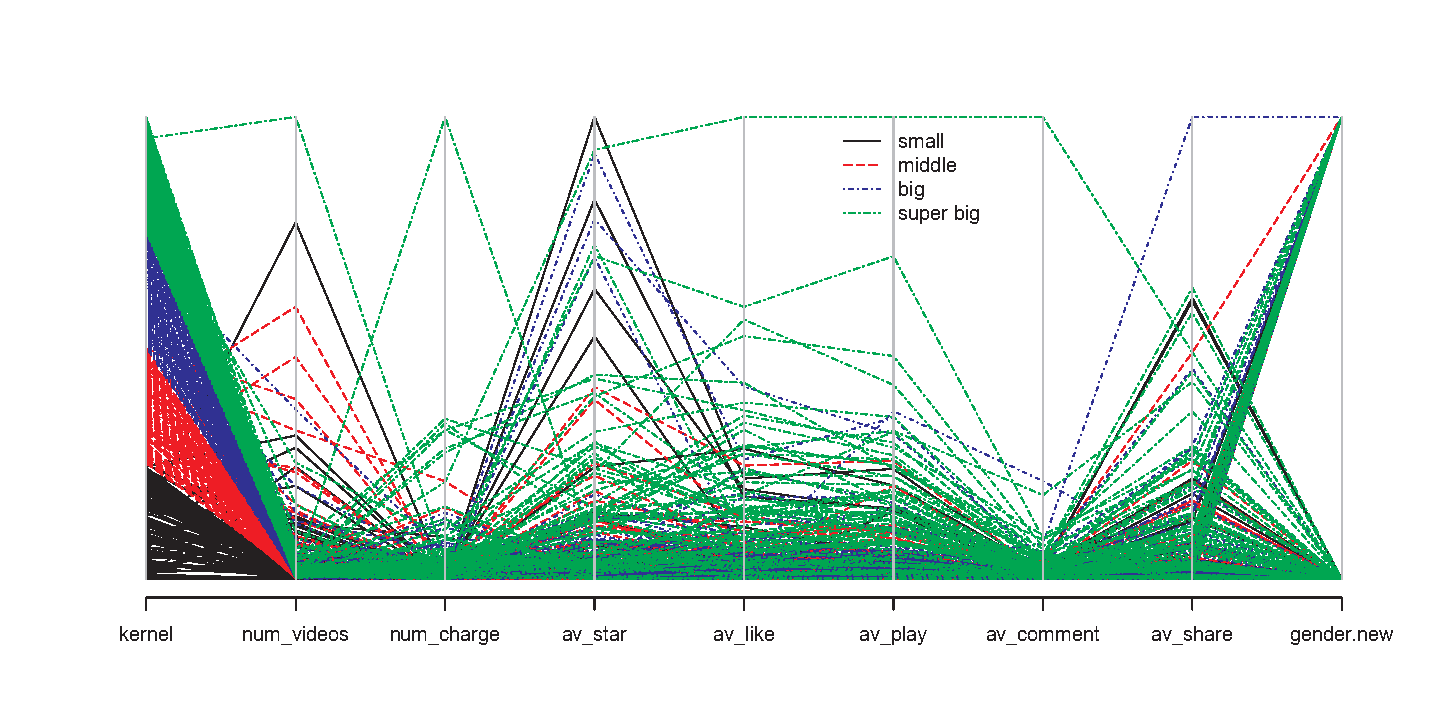
\includegraphics[width=1.0\textwidth]{MLR/Figure_parcoord.png}
    \caption{并行坐标图}
\end{figure}

\subsection{建立模型}

由于响应变量Y是ordinal的,记响应变量fans\_cat为Y,四个粉丝量级与Y的对应关系为:
small(Y=1)<middle(Y=2)<big(Y=3)<super big(Y=4),我们对各水平的累积概率的logit
采用相同的斜率,即采用“平行”的累积逻辑回归模型,模型如下:
\begin{equation}
    \operatorname{logit}(P(Y\le j))=\alpha_j+\beta_1x_1+\cdots+\beta_px_p,\ j=1,2,3
\end{equation}


将响应变量和8个解释变量放入R中得到最初模型,其Anova如下图所示,可以看到性别、视频数量和近期视频平均评论数
这3个解释变量对应的系数均不显著。
\begin{figure}[H]
    \centering
    \begin{minipage}[t]{0.48\textwidth}
        \centering
        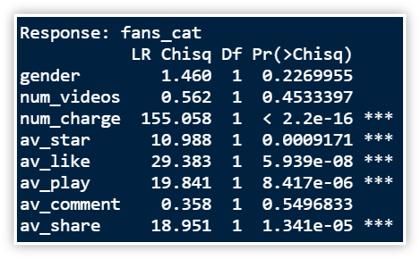
\includegraphics[width=\textwidth]{MLR/Anova1.png}
        \caption{Anova of first model}
    \end{minipage}
    \begin{minipage}[t]{0.48\textwidth}
        \centering
        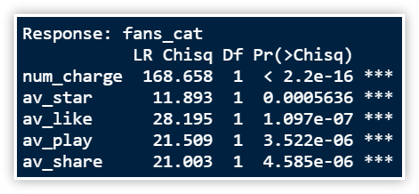
\includegraphics[width=\textwidth]{MLR/Anova2.png}
        \caption{Anova of final model}
    \end{minipage}
\end{figure}


采用Backward Elimination的变量选取方法,并以AIC为准则,可以依次去除近期评论数,
视频数,性别这3个解释变量,将剩余5个解释变量拟合得到最终模型,从图12可以看到
最终模型中5个解释变量均显著。

\subsection{模型解释}

利用R中的vglm函数得到最终的估计模型如下:
\begin{equation*}
    \operatorname{logit}(\hat{P}(Y\le j))=\hat\alpha_j-29.4num\_charge+16.8av\_star-48.6av\_like-19.4av\_play+15.6av\_share
\end{equation*}

其中$\hat\alpha_1=-0.2,\hat\alpha_2=1.3,\hat\alpha_3=2.9$

我们注意到估计模型中$\beta_{num\_charge},\ \beta_{av\_like}, \beta_{av\_play}$均小于0,
说明num\_charge,av\_like,av\_play高的up主更倾向于是量级高的UP主,而
$\beta_{av\_star},\ \beta_{av\_share}$均大于0,说明av\_star和av\_share
高的UP主倾向于是量级低的UP主,这似乎与直觉不太相符,但由于这只是近8个视频的指标,所以
我们可以猜测这些视频可能只是通过“玩梗”等方式在短期获得了较大的关注,或者是新UP主。


结合整个建模过程的分析,我们可以得到以下结论:

(1) 首先性别变量不显著,说明UP主粉丝数量级可能与性别关系不大.

(2) 一些高质量视频的正向收益指标(点赞数,充电数)显著,而总视频数并不显著,
说明相较于视频数量,UP主粉丝数量级与其视频质量的关系更大。说明想成为一名
大Up主,视频在精不在多.

(3) 从拟合模型的系数上看,充电量、点赞量、播放量高的更倾向于是量级高
的UP主,而近期视频收藏量,分享量高的更可能是“昙花一现”。

\subsection{数据可视化}

为了便于数据可视化,我们系数最显著的解释变量充电量num\_charge单独拟合累积逻辑
回归模型得到概率估计图如下,左侧是各个粉丝量级的概率分布,右侧是粉丝数量级的累
积概率。

\begin{figure}[H]
    \centering
    \begin{minipage}[t]{0.48\textwidth}
        \centering
        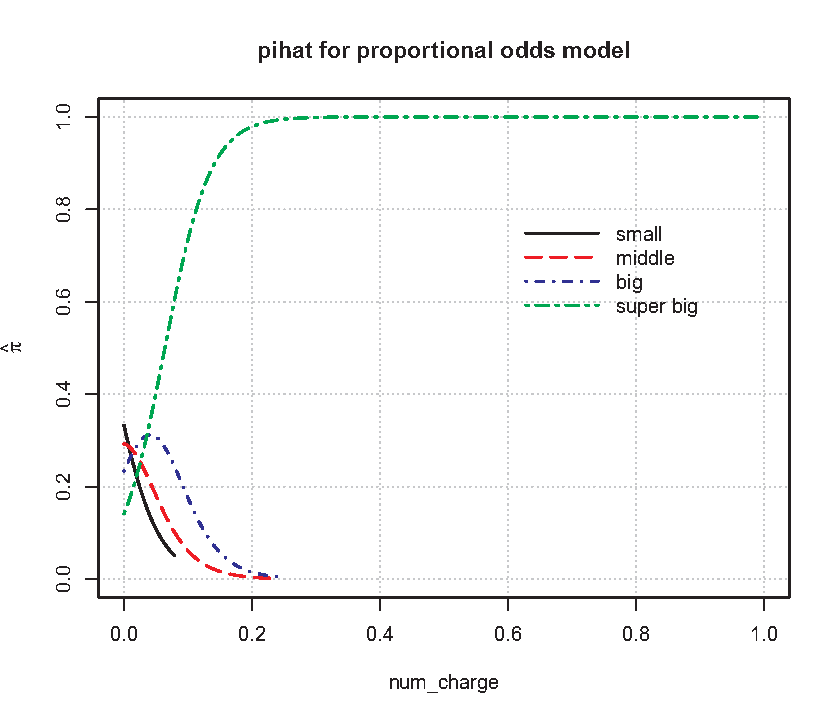
\includegraphics[width=\textwidth]{MLR/Figure_propotional.png}
    \end{minipage}
    \begin{minipage}[t]{0.48\textwidth}
        \centering
        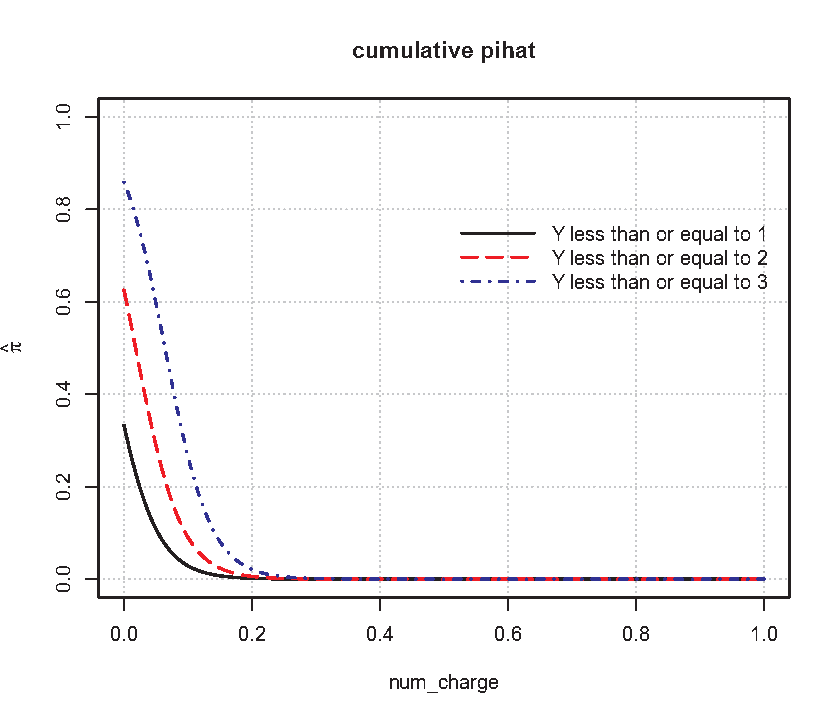
\includegraphics[width=\textwidth]{MLR/Figure_cumulative.png}    
    \end{minipage}
    \caption{以充电量为解释变量的累积逻辑回归模型概率分布图和累积概率图}
\end{figure}


从左图中我们可以看出充电量在超级大UP主和非超级UP主之间分布非常不均匀,归一化后
的充电量约为0.23以上时,UP主是超级UP主的概率就为1了;从右图可以看出并且随着充
电量的增加,小,中,大量级对应的累积概率都递减,说明充电量稍微大一些,就很可能
是超级UP主了,换言之,归一化后0.23充电量以上的UP主中基本都是超级UP主,这也反映
了一种超级UP主和非超级UP主之间的“贫富差距”大的两极分化现象。

事实上,我们本身抽取UP采用回溯性研究,每个量级的UP主都抽取了250位,但实际上100万
粉以上的超级UP主的数量相较于100万粉以下的小中大UP主的数量是少得可怜的(列联表部分
给出数据),但在抽取数据中充电量23\%值最大值以上都是超级UP主,而充电量本身就是UP主
获得收益的一个主要渠道之一,可见少数的头部UP主获得远多于非头部UP主的收益,这体现了
B站UP主的一种金字塔效应。

\subsection{模型改进}

在多分类逻辑回归分析部分,我们使用了“平行”的累积回归模型,对于最初的8解释变量
模型,AIC=2273.2;对于最后的5解释变量模型,AIC=2269.1。我们发现最终得到的模型
的AIC依旧在2000以上,说明模型并不是很理想。我们知道,在使用“平行”的累积回归模型
时,我们假定了各解释变量对响应变量各水平的累积变量的影响是一致的,这个假设是否
太强了,导致模型拟合不佳?我们因此尝试了“非平行”的累积逻辑回归模型,当解释变量
为8个时,“非平行”逻辑回归模型的$3\times(8+1)=27$的参数均显著,但是注意到“非平行”
模型的Log-likelihood为NA,经过查阅资料和分析发现,在“非平行”模型情况下出现了累积
概率“交叉”的情况,此时各粉丝量水平概率估计值出现负值,因此导致模型失效,因此“非平
行”模型在本数据中不适用。

我们可以采取多项累积回归模型作为“非平行”累积回归模型的一种替代,看看是否复杂一
些的模型有更好的效果,模型如下:
\begin{equation}
\begin{aligned}
    \log(\pi_j/\pi_{small})=\alpha_j+\beta_{j1}x_1+\cdots+\beta_{jp}x_p, j=middle,big,super\ big\\
\end{aligned}  
\end{equation}

经过Anova分析(下图左)发现模型的视频数变量不显著,建立去除后视频数的模型,进行卡方检验,
p-value=0.44,说明可以保留简便的模型,即去除视频数的模型,我们由此得到一个7
解释变量的模型,得到的Anova表(下图右)中所有变量均显著。

\begin{figure}[H]
    \centering
    \begin{minipage}[t]{0.48\textwidth}
        \centering
        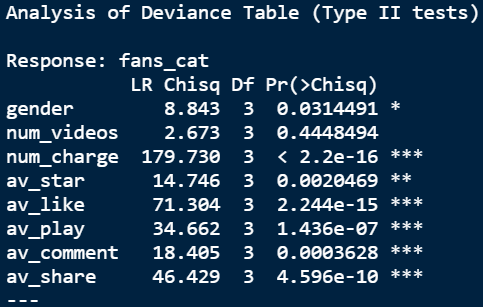
\includegraphics[width=\textwidth]{MLR/AnovaMul1.png}
        \caption{Anova of first model}
    \end{minipage}
    \begin{minipage}[t]{0.48\textwidth}
        \centering
        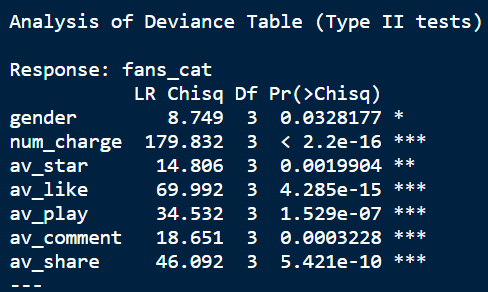
\includegraphics[width=\textwidth]{MLR/AnovaMul2.png}
        \caption{Anova of final model}
    \end{minipage}
\end{figure}

得到的多项逻辑回归模型估计系数如下:

\begin{table}[H]
    \centering
    \begin{tabular}{ccccccccc}
        \toprule
          & Intercept & gender & num\_charge & av\_star
          & av\_like & av\_play & av\_comment & av\_share\\
        \midrule
          $\log(\frac{\hat\pi_{middle}}{\hat\pi_{small}})$ 
          & -0.7 & -0.5 & 58 & -12
          & 84 & 8.0 & -5.1 & -22\\
          $\log(\frac{\hat\pi_{big}}{\hat\pi_{small}})$
          & -1.3 & 0.01 & 61 & -27
          & 121 & 18 & 13 & -42\\
          $\log(\frac{\hat\pi_{super big}}{\hat\pi_{small}})$
          & -2.7 & -0.1 & 81 & -28
          & 129 & 39 & 1.5 & -46\\
        \bottomrule
     \end{tabular}
    \caption{多分类逻辑回归解释变量}
\end{table}

从上表中我们可以得到分析如下:

(1) 由于解释变量是归一化的,系数的绝对值可以一定程度反映解释变量对
响应变量不同分类之间odds的影响,在3个水平下,性别和近期平均评论数
的系数绝对值均较小,说明它们对响应变量影响较小,这与累积逻辑回归模
型部分的结果是一致的。

(2) 充电数和近期平均点赞数的系数在3个level下为正且较大,说明随着充电
数和近期平均点赞数的增大,UP主位于中、大、超级UP主相较于小UP主的odds
均增大,并且这种增大的效应比较显著。同时充电数和近期平均点赞数的系数
满足super big>big>middle,说明这种odds的增大效应随着UP主量级的增大
而增大。

(3) 近期平均收藏量,近期平均分享量的系数为负,随着近期平均收藏量,近
期平均分享量的增大,UP主位于中、大、超级UP主相较于小UP主的odds均减小,
这也与直觉不太相符,我们在累积逻辑回归部分已试图分析过其原因。

最终得到的多项逻辑回归的AIC=2208.4,略优于“平行”的逻辑回归模型,但也
并不太理想。并且从可解释性上看,似乎引入这种更为复杂的模型并没有给我们
带来更多的可解释性,因此综合各方面看,我们认为采用“平行”逻辑回归模型来
刻画UP主粉丝数的分类与各视频指标的关系是最优的。

\section{研究结论}

经过实际情况与以上的数据分析,我们可以总结出三点成为B站头部up主的秘诀。

(1)首先是要尝试自己擅长的领域,因为想要成为一名顶尖up主更多取决于视频
质量的高低而非视频数量的多少,而在自己擅长的领域更容易做出高质量的视频。

(2)如果不知道成为哪个区的up主更容易收获粉丝,我们建议你可以从游戏区开
始,因为游戏区的投递视频门槛相对较低,游戏选择合适的话更容易吸引对应
玩家群体观看。

(3)要保证视频质量持久稳定而非“昙花一现”,这样才能收获长期支持的真爱
粉,足够多的真爱粉使视频保持长期持久的关注度,这将是成为头部up主的基
础。

\section{研究缺陷与改进}

\subsection{分区方式}

在列联表研究中,我们只选择了三个分区为代表进行研究。我们的本意是想要建立有关全部分区的研究,但是受制于
我们抽取数据的方式,如果直接进行更多分区的列联表研究,会有同一个UP主同时设计多个分区的情况,尤其在粉丝量
大的部分,重复比例会相当严重,从而造成研究的结果不准确。因此我们尽量选择了重合较少的UP主进行分类数据处理,
让分析的结果尽量准确。\\
\indent 因此,在后续可以考虑优化数据获取的方式,如爬下所有数据后进行去重(但我们抽取数据的网站对其有限制)等
更加优化的抽取数据方式,来得到更多分区下的联表研究。\\
\indent 同时,从EDA中可以看出,可能粉丝量的分类存在一定不合理的方式,因为在粉丝量较小的情况下,UP主的各个
指标没有表现出明显的差异,因此放入模型中会让模型较为不显著,在回归时也会降低回归的效益。因此后续可以通过调整
如何对粉丝量进行分区,来找到UP主的粉丝量的更显著的“台阶”。

\subsection{多分类回归与线性回归}
从LASSO的结果可以看出,多分类回归和线性回归得到的系数是不同的,因此这提示我们在进行粉丝量分区处理时,出现了
一定的信息损失,或者说变异。从解释性上,可以说是由于粉丝量上一层与在全区间意义下的粉丝量的提升相关的变量存在
不同重要性的影响因素。但是这种信息造成的偏差也是值得注意的。\\
\indent 进行了线性回归分析后,发现直接的线性回归对数据的拟合并不好,因此为更好地拟合相关的数据,可以考虑效益
更加强的其它方法进行数据的处理。\\
\indent 当然,也应该发现的是其实二者的相似性还是比较强的,比如线性回归被正则的参数在多分类逻辑回归中的效益
也较低,最后在筛选变量后被去除。因此也一定程度上说明了此种分类方式后的逻辑回归和不分类的线性回归有较强的相同的效益。

\section*{分工与致谢}

在本次大作业中,周子逸负责数据的爬取和清洗,徐智昱负责数据预处理,EDA以及研究缺陷和改进部分,逄一哲负责
列联表分析部分,祝尔康负责多分类逻辑回归部分及论文整合,4位同学都参与了pre的准备以及论文的撰写。

最后,感谢王江典老师和王梓涵助教对本次大作业的指导和帮助,感谢您指引我们走进多分类数据分析的殿堂,并在百忙
之中为我们的研究提供指导性意见。

\end{document}